
%-----------------------------------------------------------------------------------------------------------------------------------------------%
%	The MIT License (MIT)
%
%	Copyright (c) 2019 Jan Küster
%
%	Permission is hereby granted, free of charge, to any person obtaining a copy
%	of this software and associated documentation files (the "Software"), to deal
%	in the Software without restriction, including without limitation the rights
%	to use, copy, modify, merge, publish, distribute, sublicense, and/or sell
%	copies of the Software, and to permit persons to whom the Software is
%	furnished to do so, subject to the following conditions:
%	
%	THE SOFTWARE IS PROVIDED "AS IS", WITHOUT WARRANTY OF ANY KIND, EXPRESS OR
%	IMPLIED, INCLUDING BUT NOT LIMITED TO THE WARRANTIES OF MERCHANTABILITY,
%	FITNESS FOR A PARTICULAR PURPOSE AND NONINFRINGEMENT. IN NO EVENT SHALL THE
%	AUTHORS OR COPYRIGHT HOLDERS BE LIABLE FOR ANY CLAIM, DAMAGES OR OTHER
%	LIABILITY, WHETHER IN AN ACTION OF CONTRACT, TORT OR OTHERWISE, ARISING FROM,
%	OUT OF OR IN CONNECTION WITH THE SOFTWARE OR THE USE OR OTHER DEALINGS IN
%	THE SOFTWARE.
%	
%
%-----------------------------------------------------------------------------------------------------------------------------------------------%


%============================================================================%
%
%	DOCUMENT DEFINITION
%
%============================================================================%

\documentclass[10pt,A4,german]{article}	


%----------------------------------------------------------------------------------------
%	ENCODING
%----------------------------------------------------------------------------------------

% we use utf8 since we want to build from any machine
\usepackage[utf8]{inputenc}		
\usepackage[ngerman]{isodate}
\usepackage{fancyhdr}
\usepackage[numbers]{natbib}

%----------------------------------------------------------------------------------------
%	LOGIC
%----------------------------------------------------------------------------------------

% provides \isempty test
\usepackage{xstring, xifthen}
\usepackage{enumitem}
\usepackage[german]{babel}
\usepackage{blindtext}
\usepackage{pdfpages}
\usepackage{changepage}

%----------------------------------------------------------------------------------------
%	FONT BASICS
%----------------------------------------------------------------------------------------

% some tex-live fonts - choose your own

%\usepackage[defaultsans]{droidsans}
%\usepackage[default]{comfortaa}
%\usepackage{cmbright}
\usepackage[default]{raleway}
%\usepackage{fetamont}
%\usepackage[default]{gillius}
%\usepackage[light,math]{iwona}
%\usepackage[thin]{roboto} 

% set font default
\renewcommand*\familydefault{\sfdefault} 	
\usepackage[T1]{fontenc}

% more font size definitions
\usepackage{moresize}

%----------------------------------------------------------------------------------------
%	FONT AWESOME ICONS
%---------------------------------------------------------------------------------------- 

% include the fontawesome icon set
\usepackage{fontawesome}

% use to vertically center content
% credits to: http://tex.stackexchange.com/questions/7219/how-to-vertically-center-two-images-next-to-each-other
\newcommand{\vcenteredinclude}[1]{\begingroup
\setbox0=\hbox{\includegraphics{#1}}%
\parbox{\wd0}{\box0}\endgroup}
\newcommand{\tab}[1]{\hspace{.2\textwidth}\rlap{#1}}
% use to vertically center content
% credits to: http://tex.stackexchange.com/questions/7219/how-to-vertically-center-two-images-next-to-each-other
\newcommand*{\vcenteredhbox}[1]{\begingroup
\setbox0=\hbox{#1}\parbox{\wd0}{\box0}\endgroup}

% icon shortcut
\newcommand{\icon}[3] { 							
	\makebox(#2, #2){\textcolor{maincol}{\csname fa#1\endcsname}}
}	


% icon with text shortcut
\newcommand{\icontext}[4]{ 						
	\vcenteredhbox{\icon{#1}{#2}{#3}}  \hspace{2pt}  \parbox{0.9\mpwidth}{\textcolor{#4}{#3}}
}

% icon with website url
\newcommand{\iconhref}[5]{ 						
    \vcenteredhbox{\icon{#1}{#2}{#5}}  \hspace{2pt} \href{#4}{\textcolor{#5}{#3}}
}

% icon with email link
\newcommand{\iconemail}[5]{ 						
    \vcenteredhbox{\icon{#1}{#2}{#5}}  \hspace{2pt} \href{mailto:#4}{\textcolor{#5}{#3}}
}

%----------------------------------------------------------------------------------------
%	PAGE LAYOUT  DEFINITIONS
%----------------------------------------------------------------------------------------

% page outer frames (debug-only)
% \usepackage{showframe}		

% we use paracol to display breakable two columns
\usepackage{paracol}
\usepackage{tikzpagenodes}
\usetikzlibrary{calc}
\usepackage{lmodern}
\usepackage{multicol}
\usepackage{lipsum}
\usepackage{atbegshi}
% define page styles using geometry
\usepackage[a4paper]{geometry}

% remove all possible margins
\geometry{top=1cm, bottom=1cm, left=1cm, right=1cm}

\usepackage{fancyhdr}
\pagestyle{empty}

% space between header and content
% \setlength{\headheight}{0pt}

% indentation is zero
\setlength{\parindent}{0mm}

%----------------------------------------------------------------------------------------
%	TABLE /ARRAY DEFINITIONS
%---------------------------------------------------------------------------------------- 

% extended aligning of tabular cells
\usepackage{array}

% custom column right-align with fixed width
% use like p{size} but via x{size}
\newcolumntype{x}[1]{%
>{\raggedleft\hspace{0pt}}p{#1}}%


%----------------------------------------------------------------------------------------
%	GRAPHICS DEFINITIONS
%---------------------------------------------------------------------------------------- 

%for header image
\usepackage{graphicx}

% use this for floating figures
% \usepackage{wrapfig}
% \usepackage{float}
% \floatstyle{boxed} 
% \restylefloat{figure}

%for drawing graphics		
\usepackage{tikz}			
\usepackage{ragged2e}	
\usetikzlibrary{shapes, backgrounds,mindmap, trees}

%----------------------------------------------------------------------------------------
%	Color DEFINITIONS
%---------------------------------------------------------------------------------------- 
\usepackage{transparent}
\usepackage{color}

% primary color
\definecolor{maincol}{RGB}{ 64,64,64}

% accent color, secondary
% \definecolor{accentcol}{RGB}{ 250, 150, 10 }

% dark color
\definecolor{darkcol}{RGB}{ 70, 70, 70 }

% light color
\definecolor{lightcol}{RGB}{245,245,245}

\definecolor{accentcol}{RGB}{59,77,97}



% Package for links, must be the last package used
\usepackage[hidelinks]{hyperref}

% returns minipage width minus two times \fboxsep
% to keep padding included in width calculations
% can also be used for other boxes / environments
\newcommand{\mpwidth}{\linewidth-\fboxsep-\fboxsep}
	


%============================================================================%
%
%	CV COMMANDS
%
%============================================================================%

%----------------------------------------------------------------------------------------
%	 CV LIST
%----------------------------------------------------------------------------------------

% renders a standard latex list but abstracts away the environment definition (begin/end)
\newcommand{\cvlist}[1] {
	\begin{itemize}{#1}\end{itemize}
}

%----------------------------------------------------------------------------------------
%	 CV TEXT
%----------------------------------------------------------------------------------------

% base class to wrap any text based stuff here. Renders like a paragraph.
% Allows complex commands to be passed, too.
% param 1: *any
\newcommand{\cvtext}[1] {
	\begin{tabular*}{1\mpwidth}{p{0.98\mpwidth}}
		\parbox{1\mpwidth}{#1}
	\end{tabular*}
}
\newcommand{\cvtextsmall}[1] {
	\begin{tabular*}{0.8\mpwidth}{p{0.8\mpwidth}}
		\parbox{0.8\mpwidth}{#1}
	\end{tabular*}
}
%----------------------------------------------------------------------------------------
%	CV SECTION
%----------------------------------------------------------------------------------------

% Renders a a CV section headline with a nice underline in main color.
% param 1: section title
\newlength{\barw}
\newcommand{\cvsection}[1] {
	\vspace{14pt}
	\settowidth{\barw}{\textbf{\LARGE #1}}
	\cvtext{
		\textbf{\LARGE{\textcolor{darkcol}{#1}}}\\[-4pt]
		\textcolor{accentcol}{ \rule{\barw}{1.5pt} } \\
	}
}

\newcommand{\cvsectionsmall}[1] {
	\vspace{14pt}
	\settowidth{\barw}{\textbf{\Large #1}}
	\cvtext{
		\textbf{\Large{\textcolor{darkcol}{#1}}}\\[-4pt]
		\textcolor{accentcol}{ \rule{\barw}{1.5pt} } \\
	}
}

\newcommand{\cvheadline}[1] {
	\vspace{16pt}
	\cvtext{
		\textbf{\Huge{\textcolor{accentcol}{#1}}}\\[-4pt]
		 
	}
}

\newcommand{\cvsubheadline}[1] {
	\vspace{16pt}
	\cvtext{
		\textbf{\huge{\textcolor{darkcol}{#1}}}\\[-4pt]
		 
	}
}
%----------------------------------------------------------------------------------------
%	META SKILL
%----------------------------------------------------------------------------------------

% Renders a progress-bar to indicate a certain skill in percent.
% param 1: name of the skill / tech / etc.
% param 2: level (for example in years)
% param 3: percent, values range from 0 to 1
\newcommand{\cvskill}[3] {
	\begin{tabular*}{1\mpwidth}{p{0.72\mpwidth}  r}
 		\textcolor{black}{\textbf{#1}} & \textcolor{maincol}{#2}\\
	\end{tabular*}%
	
	\hspace{4pt}
	\begin{tikzpicture}[scale=1,rounded corners=2pt,very thin]
		\fill [lightcol] (0,0) rectangle (1\mpwidth, 0.15);
		\fill [accentcol] (0,0) rectangle (#3\mpwidth, 0.15);
  	\end{tikzpicture}%
}


%----------------------------------------------------------------------------------------
%	 CV EVENT
%----------------------------------------------------------------------------------------

% Renders a table and a paragraph (cvtext) wrapped in a parbox (to ensure minimum content
% is glued together when a pagebreak appears).
% Additional Information can be passed in text or list form (or other environments).
% the work you did
% param 1: time-frame i.e. Sep 14 - Jan 15 etc.
% param 2:	 event name (job position etc.)
% param 3: Customer, Employer, Industry
% param 4: Short description
% param 5: work done (optional)
% param 6: technologies include (optional)
% param 7: achievements (optional)
\newcommand{\cvevent}[7] {
	
	% we wrap this part in a parbox, so title and description are not separated on a pagebreak
	% if you need more control on page breaks, remove the parbox
	\parbox{\mpwidth}{
		\begin{tabular*}{1\mpwidth}{p{0.66\mpwidth}  r}
	 		\textcolor{black}{\textbf{#2}} & \colorbox{accentcol}{\makebox[0.3\mpwidth]{\textcolor{white}{\textbf{#1}}}} \\
			\textcolor{maincol}{#3} & \\
		\end{tabular*}\\[8pt]
	
		\ifthenelse{\isempty{#4}}{}{
			\cvtext{#4}\\
		}
	}
	\vspace{14pt}
}


%----------------------------------------------------------------------------------------
%	 CV META EVENT
%----------------------------------------------------------------------------------------

% Renders a CV event on the sidebar
% param 1: title
% param 2: subtitle (optional)
% param 3: customer, employer, etc,. (optional)
% param 4: info text (optional)
\newcommand{\cvmetaevent}[4] {
	\textcolor{maincol} { \cvtext{\textbf{\begin{flushleft}#1\end{flushleft}}}}

	\ifthenelse{\isempty{#2}}{}{
	\textcolor{black} {\cvtext{\textbf{#2}} }
	}

	\ifthenelse{\isempty{#3}}{}{
		\cvtext{{ \textcolor{maincol} {#3} }}\\
	}

	\cvtext{#4}\\[14pt]
}

%---------------------------------------------------------------------------------------
%	QR CODE
%----------------------------------------------------------------------------------------

% Renders a qrcode image (centered, relative to the parentwidth)
% param 1: percent width, from 0 to 1
\newcommand{\cvqrcode}[1] {
	\begin{center}
		\includegraphics[width={#1}\mpwidth]{qrcode}
	\end{center}
}


% HEADER AND FOOOTER 
%====================================
\newcommand\Header[1]{%
\begin{tikzpicture}[remember picture,overlay]
\fill[accentcol]
  (current page.north west) -- (current page.north east) --
  ([yshift=50pt]current page.north east|-current page text area.north east) --
  ([yshift=50pt,xshift=-3cm]current page.north|-current page text area.north) --
  ([yshift=10pt,xshift=-5cm]current page.north|-current page text area.north) --
  ([yshift=10pt]current page.north west|-current page text area.north west) -- cycle;
\node[font=\sffamily\bfseries\color{white},anchor=west,
  xshift=0.7cm,yshift=-0.32cm] at (current page.north west)
  {\fontsize{12}{12}\selectfont {#1}};
\end{tikzpicture}%
}

\newcommand\Footer[1]{%
\begin{tikzpicture}[remember picture,overlay]
\fill[lightcol]
  (current page.south east) -- (current page.south west) --
  ([yshift=-80pt]current page.south east|-current page text area.south east) --
  ([yshift=-80pt,xshift=-6cm]current page.south|-current page text area.south) --
  ([xshift=-2.5cm,yshift=-10pt]current page.south|-current page text area.south) --	
  ([yshift=-10pt]current page.south east|-current page text area.south east) -- cycle;
\node[yshift=0.32cm,xshift=9cm] at (current page.south) {\fontsize{10}{10}\selectfont \textbf{\thepage}};
\end{tikzpicture}%
}


%=====================================
%============================================================================%
%
%
%
%	DOCUMENT CONTENT
%
%
%
%============================================================================%
\begin{document}

\columnratio{0.31}
\setlength{\columnsep}{2.2em}
\setlength{\columnseprule}{4pt}
\colseprulecolor{white}


% LEBENSLAUF HIERE
\AtBeginShipoutFirst{\Header{Lebenslauf}\Footer{1}}
\AtBeginShipout{\AtBeginShipoutAddToBox{\Header{Lebenslauf}\Footer{2}}}

\newpage

\colseprulecolor{lightcol}
\columnratio{0.31}
\setlength{\columnsep}{2.2em}
\setlength{\columnseprule}{4pt}
\begin{paracol}{2}


\begin{leftcolumn}
%---------------------------------------------------------------------------------------
%	META IMAGE
%----------------------------------------------------------------------------------------
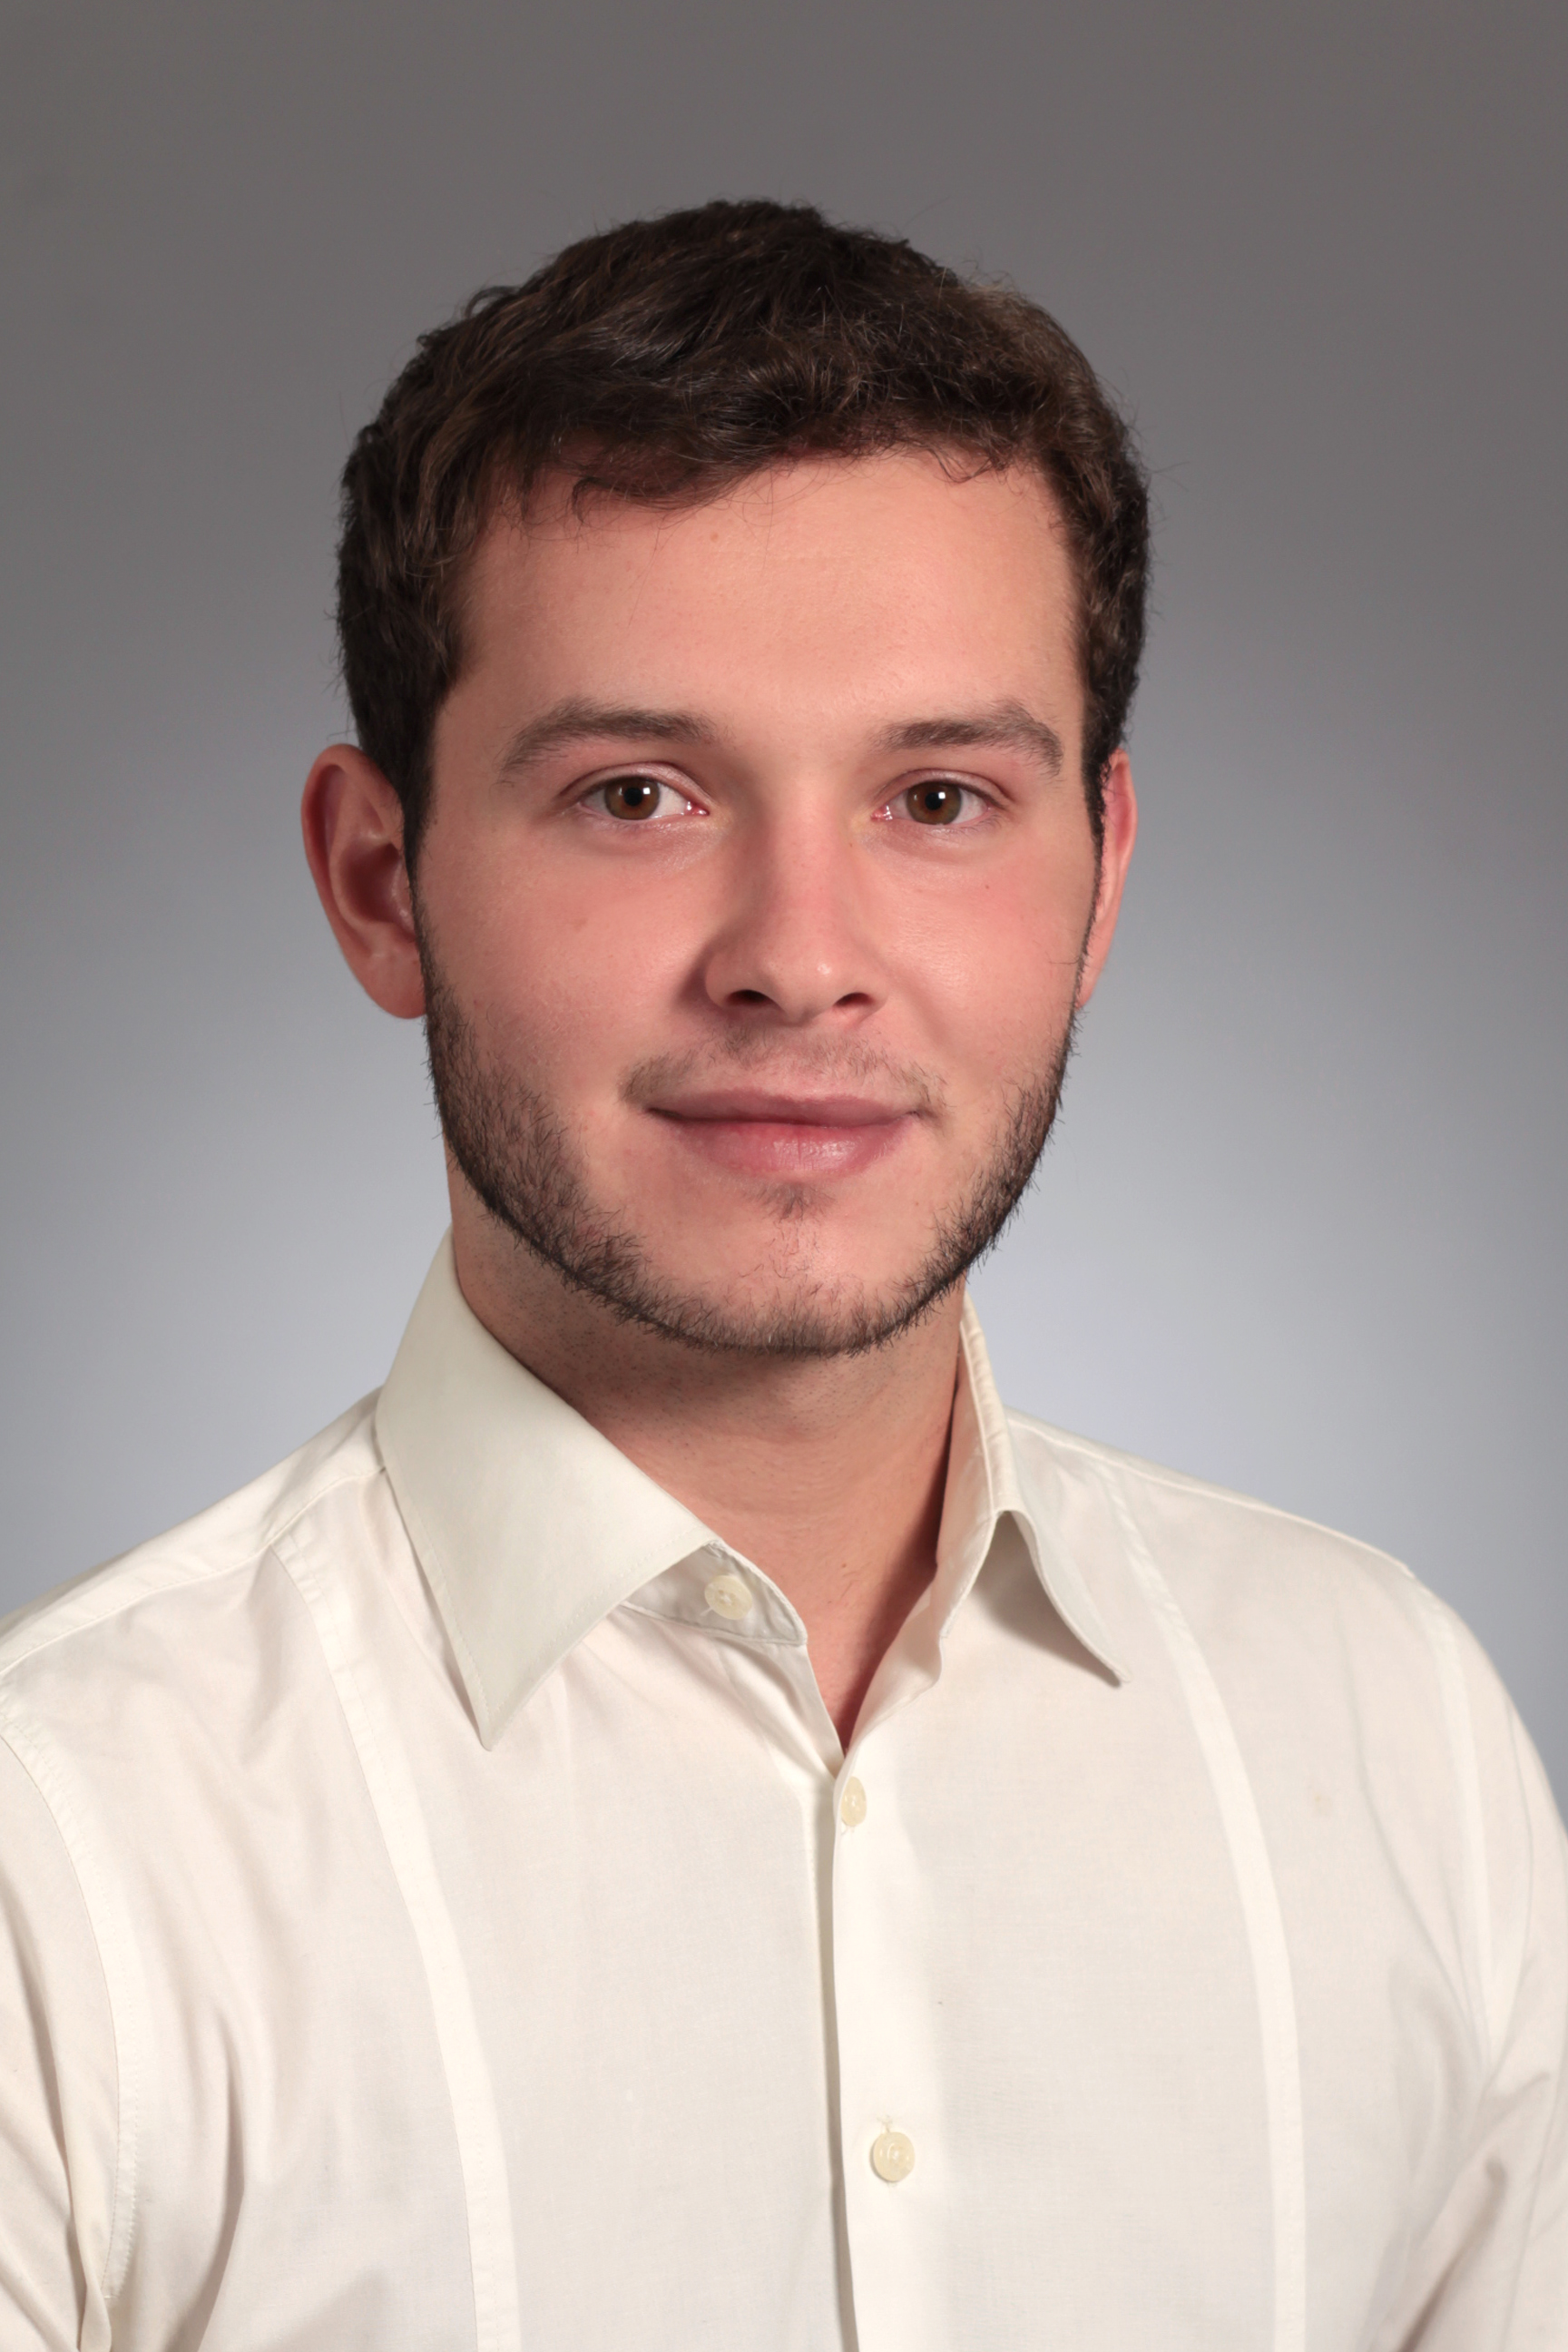
\includegraphics[width=\linewidth]{../resources/image.jpg}	%trimming relative to image size

%---------------------------------------------------------------------------------------
%	META SKILLS
%----------------------------------------------------------------------------------------
	\fcolorbox{white}{white}{\begin{minipage}[c][1.5cm][c]{1\mpwidth}
		\LARGE{\textbf{\textcolor{maincol}{Philip Empl}}} \\[2pt]
		\normalsize{ \textcolor{maincol} {Wirtschaftsinformatik (M. Sc.)} }
\end{minipage}} \\
\icontext{CaretRight}{12}{20.08.1995 in Trostberg}{black}\\[6pt]
\icontext{CaretRight}{12}{deutsch}{black}\\[6pt]
\icontext{CaretRight}{12}{ledig}{black}\\[6pt]



\cvsection{Fähigkeiten}

\cvskill{Softwareentwicklung} {6+ Jahre} {1} \\[-2pt]

\cvskill{IT-Security} {4+ Jahre} {0.64} \\[-2pt]

\cvskill{Internet Business/ \newline E-Commerce} {4+ Jahre} {0.64} \\[-2pt]

\cvskill{Webentwicklung} {2+ Jahre} {0.32} \\[-2pt]

\cvskill{Big Data/ \newline Data Science} {2+ Jahre} {0.32} \\[-2pt]

\cvskill{Distributed Legder \newline Technologie} {2+ Jahre} {0.32} \\[-2pt]

\cvskill{Internet of Things \newline (IoT)} {1+ Jahre} {0.16} \\[-2pt]

\cvskill{Cloud Computing} {1+ Jahre} {0.16} \\[-2pt] \\

\cvskill{Deutsch} {L1} {1} \\[-2pt]

\cvskill{Englisch} {C1} {0.9} \\[-2pt]

\newpage
%---------------------------------------------------------------------------------------
%	EDUCATION
%----------------------------------------------------------------------------------------
\cvsection{Bildung}

\cvmetaevent
{10/2017 - 07/2020}
{Wirtschaftsinformatik (M. Sc.)}
{Universität Regensburg}
{\textit{IT-Sicherheit • Data Science} \newline Masterarbeit: \glqq Vom Edge zur Cloud: eine explorative Studie zum Austausch und der Analyse von IoT-Daten\grqq.}
\cvmetaevent
{10/2014 - 08/2017}
{Wirtschaftsinformatik (B. Sc.)}
{Universität Regensburg}
{\textit{IT-Sicherheit • E-Commerce} \newline Bachelorarbeit: \glqq Addressing the inefficiency of searching backward: a novel tool to support authors of literature reviews\grqq.}

\cvmetaevent
{09/2006 - 06/2014}
{Allgemeines Abitur}
{Maximillian-von-Montgelas Gymnasium Vilsbiburg}
{\textit{Mathematik • Deutsch • Englisch • Wirtschaft • Musik}.}


%
%\cvsection{Projekte}

%	\cvlist{
%		\item \hyperlink{https://github.com/philipempl/ether-twin}{\textbf{Ether-Twin.}}\\ Ethereum Applikation für Digital Twins.
%		\item \hyperlink{https://github.com/philipempl/Peter-Pan}{\textbf{Peter Pan.}}\\ Koch-App (t.b.a.).
%		\item \hyperlink{https://github.com/philipempl/Innovation-Tool}{\textbf{Innovation Tool.}}\\ Webcrawler für \hyperlink{https://ibi.de/}{Ibi}.
%		\item \hyperlink{https://github.com/philipempl/cozone}{\textbf{COZONE.}} \\ Soziales Netzwerk (t.b.a.).
%		\item \hyperlink{https://github.com/geritwagner/enlit}{\textbf{ENLIT.}}\\ Exploring new Literature (Bachelorarbeit).
%		\item \textbf{Crowdfunding.} \\Modul mit \hyperlink{https://senacor.com/}{Senacor} für \hyperlink{https://www.paydirekt.de/}{paydirekt}.
%		}

\cvsection{Interessen}

\icontext{CaretRight}{12}{Gitarrist bei Edit.Sprinter}{black}\\[6pt]
\icontext{CaretRight}{12}{DIY Heimprojekte}{black}\\[6pt]
\icontext{CaretRight}{12}{Krafttraining}{black}\\[6pt]
\icontext{CaretRight}{12}{Smart Home}{black}\\[6pt]
\icontext{CaretRight}{12}{Tierschutzverein Regensburg e.V.}{black}\\[6pt]




\cvsection{Kontakt}

\icontext{MapMarker}{16}{Kumpfmühler Str. 59\\93051 Regensburg}{black}\\[6pt]
\icontext{MobilePhone}{16}{+49 152 0986 5490}{black}\\[6pt]
\iconemail{Envelope}{16}{mail@philipempl.de}{mail@philipempl.de}{black}\\[6pt]
\iconhref{Home}{16}{htifs.uni-regensburg.de}{http://www.ifs.uni-regensburg.de}{black}\\[6pt]
\iconhref{Github}{16}{github.com/philipempl}{https://www.github.com/philipempl}{black}\\[6pt]
\iconhref{Xing}{16}{xing.com/Philip\_Empl}{https://www.xing.com/profile/Philip_Empl}{black}\\

	
%\cvqrcode{0.3}

\end{leftcolumn}
\begin{rightcolumn}
%---------------------------------------------------------------------------------------
%	TITLE  HEADER
%----------------------------------------------------------------------------------------


%---------------------------------------------------------------------------------------
%	PROFILE
%----------------------------------------------------------------------------------------
\cvsection{Biographie}
\vspace{4pt}

\cvtext{Ich habe Wirtschaftsinformatik an der Universität Regensburg studiert. Meine Studienschwerpunkte waren Internet Business und Informationssicherheit im Bachelor und Informationssicherheit im Master. Seit September 2020 bin ich wissenschaftlicher Mitarbeiter am Lehrstuhl für Wirtschaftsinformatik I (Prof. Dr. Pernul). Dort bin ich an einem vom Bundesministerium für Wirtschaft und Energie (BMWi) geförderten Forschungsprojekt beteiligt. \\\\Meine Forschungsthemen sind Cybersecurity und Datenanalysen im Zusammenhang mit dem Internet of Things (IoT).}


%---------------------------------------------------------------------------------------
%	WORK EXPERIENCE
%----------------------------------------------------------------------------------------

\vspace{10pt}
\cvsection{Berufserfahrung}
\vspace{4pt}


\cvevent
{09/2020 - heute}
	{Wissenschaftlicher Mitarbeiter}
	{Lehrstuhl für Wirtschaftsinformatik I (Prof. Pernul)\newline Universität Regensburg}
	{Aufgabenbereiche: Technische Umsetzung der jeweiligen Arbeitspakete im Forschungsprojekt SISSeC und Lehre. }
	\vfill\null


\cvevent
{03/2020 - 08/2020}
	{Nebenberufliche Wissenschaftliche Hilfskraft (NWHK)}
	{Lehrstuhl für Wirtschaftsinformatik I (Prof. Pernul)\newline Universität Regensburg}
	{Aufgabenbereiche: Mitwirken im Forschungsprojekt SISSeC, das vom Bundesministeriums für Wirtschaft und Energie gefördert wird, Konzeption eines Puffer- und Persistenzsystems und Implementierung eines digitalen Zwillings. }
	\vfill\null


	
\cvevent
{09/2019 - 02/2020}
	{Tutor - IT-Security I}
	{Lehrstuhl für Wirtschaftsinformatik I (Prof. Pernul)\newline Universität Regensburg}
	{Kursinhalte: Live Hacking (SQL Injection), Klassische Kryptogaphie, Moderne Kryptogaphie (AES, DES), Kryptonanalyse, Identifikation und Authentifizierung, Rechte Management.}
	\vfill\null


	
\cvevent
    {03/2019 - 08/2019}
	{Tutor - Informationssysteme: Entwicklungen und Trends}
	{Lehrstuhl für Wirtschaftsinformatik I (Prof. Pernul)\newline Universität Regensburg}
	{Kursinhalte: Einführung in PL/SQL, Prozeduren und Funktionen, Triggerprogrammierung, Objektrelationale Erweiterungen in PL/SQL, NoSQL Grundlagen.}
	\vfill\null
	\vfill\null


   	
\cvevent
{10/2018 - 03/2019}
	{Tutor - IT-Security I}
	{Lehrstuhl für Wirtschaftsinformatik I (Prof. Pernul)\newline Universität Regensburg}
	{Kursinhalte: Live Hacking (SQL Injection), Klassische Kryptogaphie, Moderne Kryptogaphie (AES, DES), Kryptonanalyse, Identifikation und Authentifizierung, Rechte Management.}
	\vfill\null

	
\cvevent
{04/2018 - 10/2018}
	{Nebenberufliche Wissenschaftliche Hilfskraft (NWHK)}
	{Professur für Wirtschaftsinformatik (Prof. Schryen)\newline Universität Regensburg}
	{Aufgabenbereiche: Unterstützung im EPIQUALIS (Epistomologische Fortschritte durch qualitative Literature-Reviews), Erstellung von Literaturdatensätze, Statische Datenanalyse, Forschungsdokumentation, Identifikation und Authentifizierung, Verwendung von Docker, Git, Python und R.}
	\vfill\null



\cvevent
{10/2017 - 03/2018}
	{Praktikant}
	{Wertschöpfungsorientiertes Produktionssystem\newline BMW AG (Landshut)}
	{Aufgabenbereiche: Weiterentwicklung der digitalen Prozesstafel, Mitverantwortung bei dessen Rollout, Implementierung einer Rüstungscheckliste, IST-Aufnahme der Taktzeiten von Prozessen.}
	\vfill\null

\cvevent
{04/2017 - 10/2017}
	{Studentische Hilfskraft (SHK)}
	{Professur für Wirtschaftsinformatik (Prof. Schryen)\newline Universität Regensburg}
	{Aufgabenbereiche: Unterstützung im EPIQUALIS (Epistomologische Fortschritte durch qualitative Literature-Reviews), Erstellung von Literaturdatensätze, Statische Datenanalyse, Forschungsdokumentation, Identifikation und Authentifizierung, Verwendung von Docker, Git, Python und R.}
	\vfill\null


\cvevent
{10/2016 - 03/2017}
	{Tutor - Theoretische Informatik}
	{Professur für Wirtschaftsinformatik (Prof. Schryen)\newline Universität Regensburg}
	{Kursinhalte: Einführung von Automaten, Deterministische endliche Automaten, Nichtdeterministische endliche Automaten, Reguläre Ausdrücke und Sprachen, Kontextfreie Grammatik und Sprachen, Push-down Automaten, Einführung von Turing Maschinen, Entscheidungsprobleme.}
	\vfill\null



\cvevent
{03/2015 - 08/2016}
	{Werkstudent}
	{Manufacturing Executive Systems\newline DRÄXLMAIER Group (Vilsbiburg)}
	{Aufgabenbereiche: Refactoring der DTO Model Klassen im MES/ PCM Software Projekt, Tests im Rahmen des MES Rollouts, Bearbeitung diverser Issues, Wiki.}
	\vfill\null


\cvsection{Publikationen}

\begin{itemize}[leftmargin=*]
\item Wagner, G. \& Empl, P. \&  Schryen G. (2020). "Designing a novel strategy for exploring literature corpora". In: \textit{Proceedings of the 28th European Conference on Information Systems (ECIS)}, Marrakesch, June 15-17, 2020.
\end{itemize}
% hofixes to create fake-space to ensure the whole height is used
\mbox{}
\vfill
\mbox{}
\vfill
\mbox{}
\vfill
\mbox{}
\vfill
\mbox{}
\vfill
\mbox{}
\vfill
\mbox{}


Regensburg, den \today     \hspace{1cm}   \hrulefill

\hspace*{30mm}\phantom{Regensburg, den \today }Philip Empl

\end{rightcolumn}
\end{paracol}


\end{document}
